\documentclass{article}
\usepackage{tikz}
\usetikzlibrary{shapes, arrows.meta}

\begin{document}

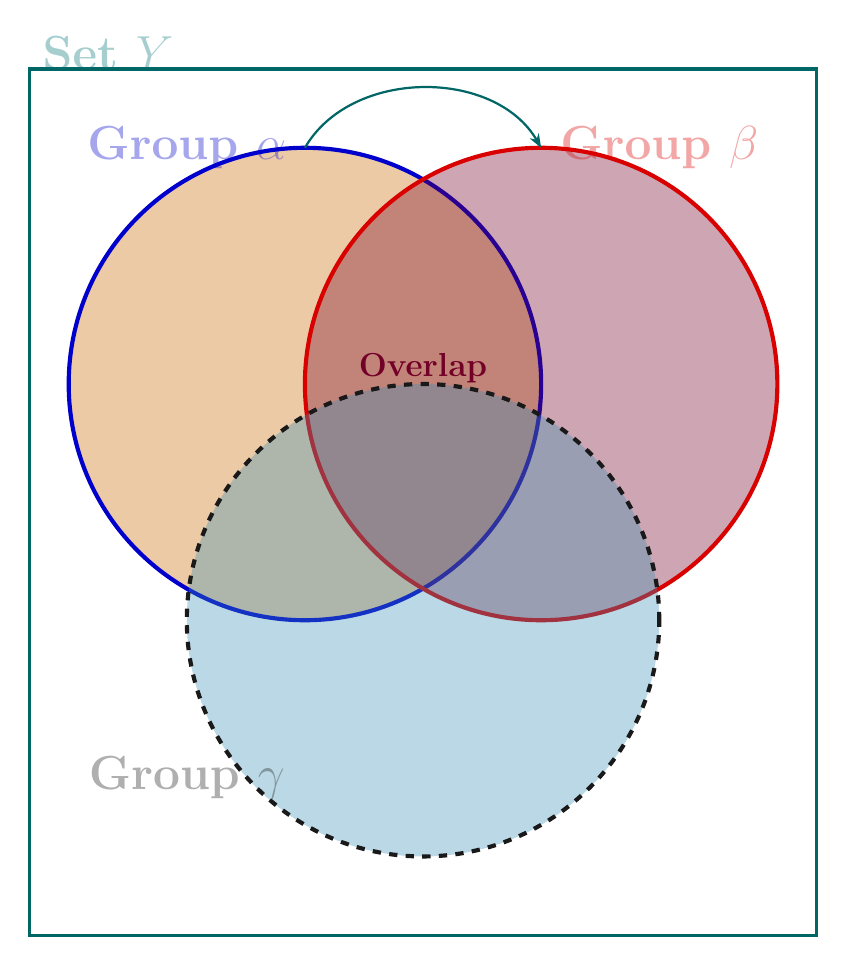
\begin{tikzpicture}
  \begin{scope}[fill opacity=0.35]
    % Rectangle border (universal set)
    \draw[line width=1.2pt, draw=teal!80!black] (-5,5) rectangle (5,-6);

    % Three circles with new colors and border styles
    \draw[fill=orange!80!black, draw=blue!80!black, line width=1.5pt] (-1.5,1) circle (3);
    \draw[fill=purple!60!black, draw=red!85!black, line width=1.5pt] (1.5,1) circle (3);
    \draw[fill=cyan!70!black, draw=gray!20!black, line width=1.5pt, dashed] (0,-2) circle (3);

    % Node labels with new names and color
    \node[font=\LARGE\bfseries, text=teal!90!black] at (-4,5.2) {Set $Y$};
    \node[font=\LARGE\bfseries, text=blue!80!black, ellipse, draw=none] at (-3,4) {Group $\alpha$};
    \node[font=\LARGE\bfseries, text=red!85!black, ellipse, draw=none] at (3,4) {Group $\beta$};
    \node[font=\LARGE\bfseries, text=gray!20!black, ellipse, draw=none] at (-3,-4) {Group $\gamma$};
  \end{scope}

  % Example relationship arrow (showing semantic connection)
  \draw[-{Stealth[length=5pt]}, thick, teal!80!black] (-1.5,4) to[out=60,in=120] (1.5,4);

  % Annotate intersection region
  \node[font=\large\bfseries, text=purple!60!black] at (0,1.2) {Overlap};

\end{tikzpicture}

\end{document}